\chapter{Pāli Text Editor}\label{chap:editor}

In this part we will examine general tools that can be used for various purposes. The first one we should know is the internal text editor. I call this \emph{Pāli Text Editor} or sometimes simply (the program's) \emph{Text Editor} or just \emph{Editor}. This is a specialized text editor for using with Roman Pāli text, especially with the text collections handled by the program.

In the main window, Text Editor is always present in the last tab. To launch a new window of it, you can use {\faSix \symbol{"F303}} and {\faSix \symbol{"F574}} button, or their equivalent in menu File. The former opens a blank window to edit a new text; the latter opens an existing file.

\dothis{To open a new window of Text Editor:\\
\hspace{5mm}\bullet\ Click {\faSix \symbol{"F303}} button to open a new window\\
\hspace{5mm}\bullet\ Or use menu File > {\faSix \symbol{"F303}} Edit a new text file\\
\hspace{5mm}\bullet\ Click {\faSix \symbol{"F574}} button to open a file\\
\hspace{5mm}\bullet\ Or use menu File > {\faSix \symbol{"F574}} Open a text file\\
}

Figure \ref{fig:editor-blank} shows a blank window of Editor when newly opened. By default, it uses the regular mode of input (\fbox{a\blacktriangleright a}), meaning the normal input mode of your computer. If you want to type in Pāli text, you may have to change the mode to \fbox{x\blacktriangleright ā} or \fbox{ā\blacktriangleright ā} by clicking the button (or press \texttt{Ctrl-Space}). The explanation on Pāli input methods can be found in Section \ref{sect:pali-input} on page \pageref{sect:pali-input}.

\begin{figure}[!hbt]
\centering
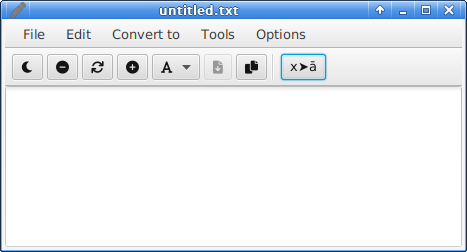
\includegraphics[width=0.8\linewidth]{images/editor-blank.png}\\
\caption{A new window of Pāli Text Editor}
\label{fig:editor-blank}
\end{figure}

Comparing the Editor with other text editors in your computer, it may not be so powerful or enjoyable to use regularly. To handle Pāli text, however, this tool is quite helpful because it has functions absent in most text editors. The first one as we have seen is the Editor has comfortable ways to enter Pāli letters. Other useful functions will be explained in the following sections. Some common functions of text editors will be left out, though.

\boxcaveat{Opening a large text file in Pāli Text Editor will make it considerably sluggish.}

\section{Find and replace}

Finding a string in a text file is a basic function of an editor. In the Editor, you can use this function by pressing \texttt{Ctrl-F} or by menu Edit > Find. When you see the find dialog, simply enter a string (mind the input mode mentioned above) and a result will be highlighted. The search is incremental. Figure \ref{fig:editor-find-simple} shows a simple finding.

\begin{figure}[!hbt]
\centering
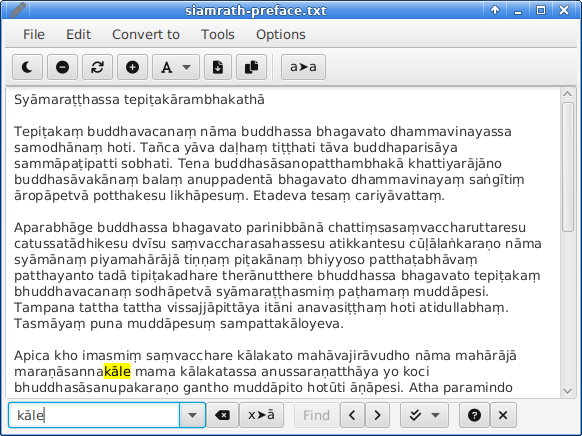
\includegraphics[width=0.9\linewidth]{images/editor-find-simple.png}\\
\caption{Finding a string in a simple way}
\label{fig:editor-find-simple}
\end{figure}

To highlight the next or previous occurrence, if any, press the Next ({\faSix \symbol{"F105}}) or Previous ({\faSix \symbol{"F104}}) button accordingly. Using \texttt{Ctrl-G} and \texttt{Ctrl-Shift-G} is more convenient and faster.

\dothis{It is faster to use \texttt{Ctrl-G} and \texttt{Ctrl-Shift-G} to go to the next and previous occurrence of the findings. You may search in just one direction because the result is circular.}

There are three options to refine the search function: (1) case sensitivity, (2) whole-word matching, and (3) using regular expressions. These options can be selected by {\faSix \symbol{"F560}} menu button. Figure \ref{fig:editor-find-wholeword} shows a finding in whole-word mode. As the example shows, the whole-word matching finds the word as a separate term, not in a compound.

\newpage
\begin{figure}[!hbt]
\centering
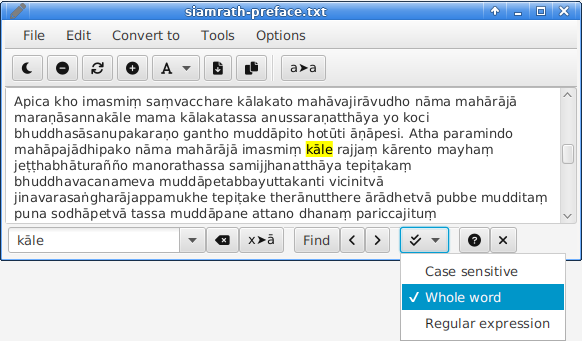
\includegraphics[width=0.9\linewidth]{images/editor-find-wholeword.png}\\
\caption{Finding a string in whole-word mode}
\label{fig:editor-find-wholeword}
\end{figure}

To obtain the same result, you can use a regular expression, as shown in Figure \ref{fig:editor-find-regexp}. Technically, the whole-word matching is a special case of regular expressions. You can in fact enter a regular expression in the whole-word mode, but avoid doing so because it will make things confusing. If a pattern is needed, use regular-expression mode (for more information, see Chapter \ref{chap:regexp}).

\begin{figure}[!hbt]
\centering
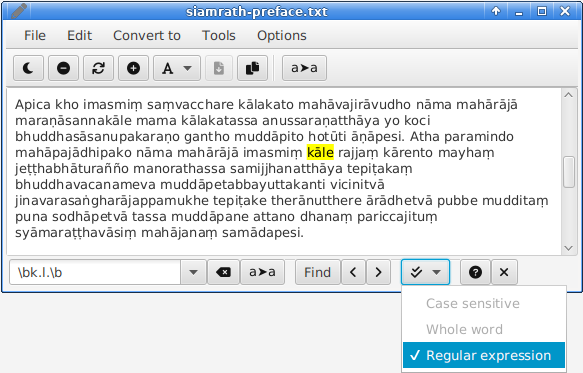
\includegraphics[width=0.9\linewidth]{images/editor-find-regexp.png}\\
\caption{Finding a string in regular-expression mode}
\label{fig:editor-find-regexp}
\end{figure}

When you edit a text file, you may need find-and-replace functionality. You can do this in the Editor in a simple way. To open the replace widget, press \texttt{Ctrl-Shift-F} or use menu Edit > Replace. When replacing a string, you may do it all at once or an instance at a time. The tool is self-explained, so I will not show you the picture. Please try it yourselves.

\section{Script transformation}

Another handy tool in the Editor is script transformation. From a Roman text file, you can convert it to the following scripts: Devanagari, Khmer, Myanmar, Sinhala, and Thai, as shown in menu Convert to (see Figure \ref{fig:editor-convert-menu}).

\begin{figure}[!hbt]
\centering
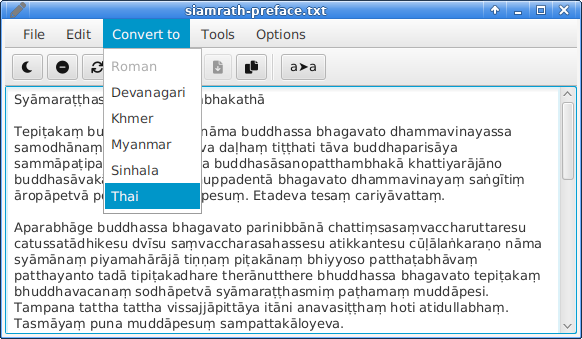
\includegraphics[width=0.9\linewidth]{images/editor-convert-menu.png}\\
\caption{Menu of script transformation}
\label{fig:editor-convert-menu}
\end{figure}

When a script language is selected, a new window of Editor will be opened with the text in that script. Figure \ref{fig:editor-convert-thai} shows a result of Thai conversion. If an external font (see Section \ref{sect:fonts} on page \pageref{sect:fonts}) is not bundled, a fallback system font will be used (see the picture). If any font is available, you can select it by {\faSix \symbol{"F031}} menu button.

\newpage
\boxnote{Roman script can be converted to other scripts, but other scripts can be converted to only Roman, except Myanmar, which can only undergo one-way conversion.\\
\hspace{5mm}Once a file is shown in a non-Roman script, you can enter or edit the file in that script with your system input method. However, the Editor is not designed to facilitate non-Roman script editing.\\
\hspace{5mm}\caveat Myanmar script conversion is very fragile. It is likely to have unexpected results.\footnote{Even the computer I use to write the program cannot display texts in Myanmar script correctly. That is why I cannot show you a picture here.} DO NOT use the text converted to Myanmar elsewhere.
}

\begin{figure}[!hbt]
\centering
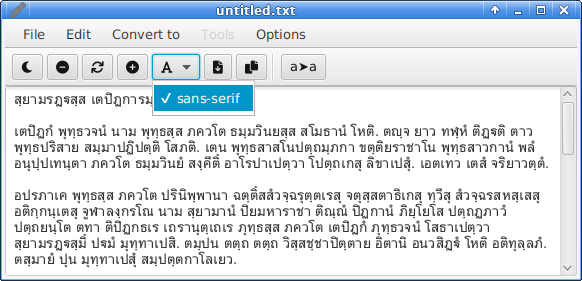
\includegraphics[width=0.9\linewidth]{images/editor-convert-thai.png}\\
\caption{Script conversion to Thai}
\label{fig:editor-convert-thai}
\end{figure}

\section{Other tools}

Apart from the two main functions described so far, the Editor can do a lot of things concerning (Roman) Pāli, as shown in the menu (see Figure \ref{fig:editor-tools-menu}). 
Most of them are obvious and need no explanation. You just spend your time playing around to get familiar with them.

\begin{figure}[!hbt]
\centering
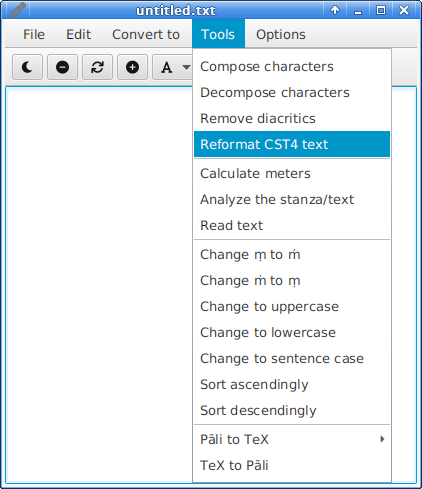
\includegraphics[width=0.5\linewidth]{images/editor-tools-menu.png}\\
\caption{Tools in the Editor}
\label{fig:editor-tools-menu}
\end{figure}

One function I have to point out to make you aware of it is the capability to reformat CST4 texts to English style of capitalization and period insertion.\footnote{The conversion is not perfect but as close as I can do. It is nonetheless better than that of the CST4.1 program or in the CSTR collection, I think.} You may need this when you use a portion from this collection because the text's format is closer to the Devanagari source. Figure \ref{fig:editor-tools-reformat} shows a result of this reformatting.

To conclude with one caveat, some operations are undoable (restorable to the previous state), particularly when you operate on a selected portion of text, but some are not (even with selected text). So, it is advisable to save you document before you use any tool, unless you are familiar well with the behavior of the actions. Some critical operations do not make change to the original text. They create new text in a new Editor instead. Script conversion is a marked example. The Editor also has options on wrapping text and its exit conditions. Please learn them privately.

\newpage
\boxnote{Notes on Pāli sorting\\
\hspace{5mm}\bullet\ To sort words, you have to put them into a list, one item per line, before you use the function.\\
\hspace{5mm}\bullet\ Sorting in Pāli uses the algorithm applied everywhere in the program. The order is fixed in the traditional way: \pali{Niggahita} (ṃ) is treated as a consonant (not vowel), so it is placed at the last position (not the position before consonants like in most dictionaries).
}

\begin{figure}[!hbt]
\centering
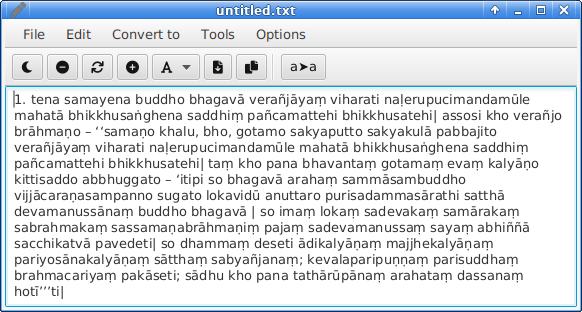
\includegraphics[width=0.9\linewidth]{images/editor-reformat-before.png}\\
(a) A portion of CST4 text\\[3mm]
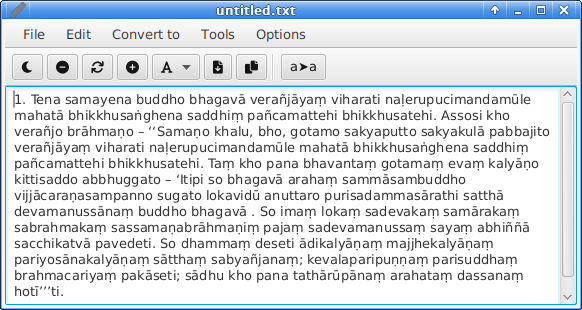
\includegraphics[width=0.9\linewidth]{images/editor-reformat-after.png}\\
(b) After reformatted\\
\caption{Reformatting of CST4 text}
\label{fig:editor-tools-reformat}
\end{figure}

